\section{Brief Overview}

In this section, some brief overview will be given for the data, as well as some pre-processing and analysis.

One thing we wanted to explore from the data, is how the points are related to one another, through principal component analysis, and clustering. Using k-means clustering, with $k = 3$, we obtained the following figure.

\begin{figure}[H] %h forces the figure to be inserted right here
    \centering
    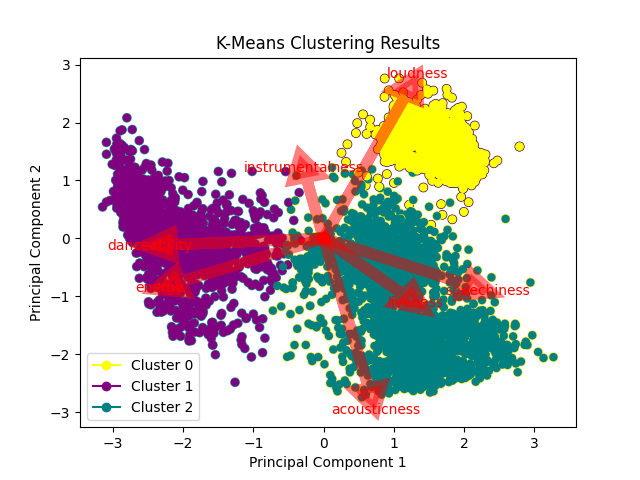
\includegraphics[width=1\linewidth]{kmeanscluster.png}
    \caption{Clustering Results}
\end{figure}

Looking at the figure, we can see that Principal Component 1 separate songs with higher liveness, speechiness, and loudness, and those with lower danceability and energy (these mostly belong to Cluster 0 and 2), and Principal Component 2 separate songs with higher instrumentalness, loudness, and those with lower acousticness (these mostly belong to Cluster 2). Overall, we can see that Cluster 0 has songs that are higher in loudness, speechiness, and liveness. Cluster 1 has songs that are lower in danceability and energy. Cluster 2 has songs high in speechiness, liveness, acousticness, but lower in instrumentalness.